
\section{Introdução}




\noindent \begin{minipage}[c]{0.6\textwidth}
  \vspace {1cm}
  \begin{description}
    \item [CloudSim] De acordo com \citeonline{cloudSim}, é um framework para simulação de infraestrutura e serviços de computação em nuvem.
    É uma opção de aprendizado vastamente utilizado pelas universidades ao redor do globo, e uma framework de código aberto e qualquer um pode contribuir com a mesma através de seu repositório no \href{https://github.com/Cloudslab}{GitHub}.
    \item [Apache NetBeans]  O NetBeans é um software de desenvolvimento integrado (IDE), sobre distribuição da licença Apache, versão 2.0, o projeto conta com código aberto e recebe contribuição de qualquer desenvolvedor que se proponha a ajudar através do \href{https://github.com/apache/netbeans-website/blob/master/netbeans.apache.org/src/content/index.adoc}{GitHub}.
\newline
    \par Site do software: \href{https://netbeans.apache.org/}{Apache NetBeans}
  \end{description}

\end{minipage}
\begin{minipage}[c]{0.4\textwidth}

  
\includegraphics[width=\textwidth]{figure/netBeana.png}
  	\label{fig:netBeans}
    \captionof{figure}{NetBeans, \cite{netBeans}}
    %\captionof*{figure}{Fonte: \citeonline{linux:2023}}
\end{minipage}

\section{Métodos}
\par Para os a elaboração da aula prática foi seguido o roteiro e um video explicativo, disponibilizado pelos professores orientadores.
\par Para este caso expecífico não foi preciso atualizar o pacote \href{https://www.oracle.com/java/technologies/downloads/}{Java JDK}, no entento necessitei baixar o \href{https://netbeans.apache.org/download/nb19/}{NetBeans 18} e o \href{https://github.com/Cloudslab/cloudsim/releases}{CloudSim 2.1}, friso que o CloudSim possui versões novas (v6.0), porém foi sugerido que usássemos a versão 2.1.

\par Para início da elaboração desta aula prática, foi prosseguido com a criação de um novo projeo na IDE NetBeans\ref{fig:netBeans}, conforme demonstrado nas figuras:\ref{fig:creat_project},\ref{fig:creat_project_name}

\begin{figure}[H]
    \center
    \subfigure[ Criação do projeto.\label{fig:creat_project}]{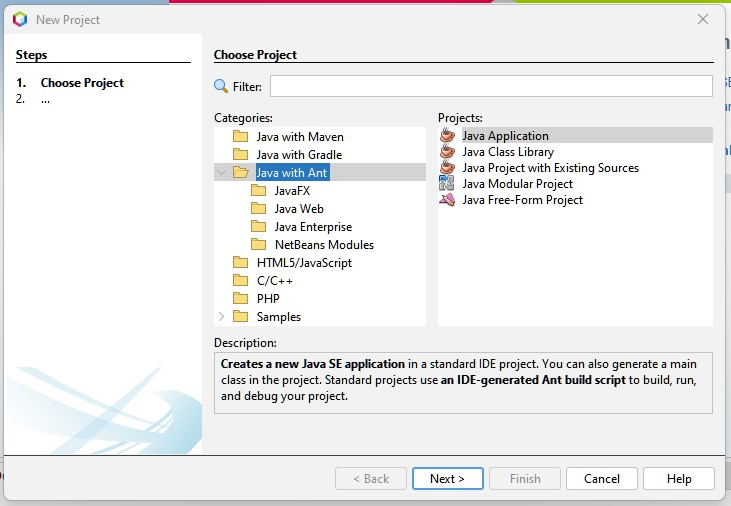
\includegraphics[scale=0.5]{figure/create_project.jpg}}
    \subfigure[Definição do nome do projeto.\label{fig:creat_project_name}]{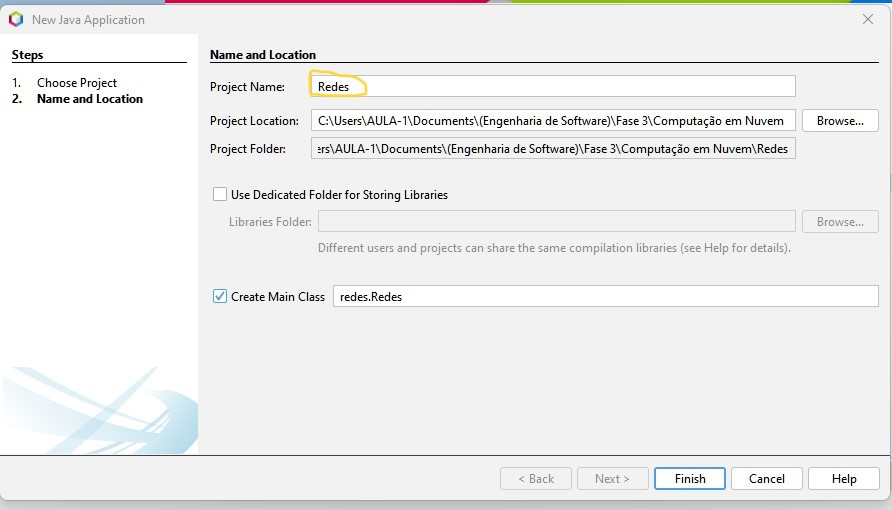
\includegraphics[scale=.5]{figure/create_project_name.jpg}}
    \caption{Etapas para a criação do projeto na IDE, O autor}\label{fig:confi_project}
\end{figure}
\par Como sugestão do roteiro o nome do projeto, foi definido como: \verb#Redes#, como demonstrado na Figura \ref{fig:creat_project_name}.




\section{Resultados}
\par De acordo com \citeonline{cloudSim:tutorial}, o que impulsiona o mecanismo de simulação central do CloudSim é o pacote que posui no dir: \verb#org.cloudbus.cloudsim.core#, com a explanação de uma fração do código vemos

\section{Conclusões}


\section{APAGAR}

\begin{figure}[H]
  \center
  \subfigure[ Algoritmo.\label{fig:pri2}]{
\includegraphics[scale=0.4]{figure/placeholder.jpg}}
  \subfigure[Comportamento.\label{fig:seg2}]{
\includegraphics[scale=.4]{figure/placeholder.jpg}}
  \caption{Resultado da atividade prática 1.2, \cite{oliveira_SO2009}}\label{fig:ap1_cod_vigual1}
\end{figure}

%%%%%%%%%%%%%%%%%%%%%%%%%%%%%%%%%%%%%%%%%%%%%%%%%%%%%%%%%%


Para referenciar utilize \cite{ninguem2022curioso}. Também pode ser citado integrada ao texto, de acordo com \citeonline{alguem2022nada}.




\begin{enumerate}[label=\Roman{*}, ref=(\roman{*})]
  \item fsfsdf
  \item kugfhiuh
\end{enumerate}

\begin{asparaenum}
\item Anterior ... \cite{ninguem2022curioso}
\item Próximo ... \label{pl1}
\end{asparaenum}


  %$X \xLongleftarrow[\text{NATAN}]{\text{OGLIARI}} Y $ %COM TEXTO
	% $\uparrow$ %Seta para Cima
	%$\overleftarrow{NATAN}$
